\section{WC 16/6/25}

\subsection*{Overview:}
This week I spent some time testing every feature ruthlessly and implementing improvements before my launch next week 

\subsection*{Achievements, Thoughts and Ideas:}
Whilst testing each feature I came across a few areas where improvements could be made

Firstly I found that the toolbar of options on both the whiteboard and document notes types, whilst perfectly functional on desktop, on mobile and smaller screens would 'wrap' around the screen - potentially covering the content users are working on. 

\begin{figure}[H]
    \centering
    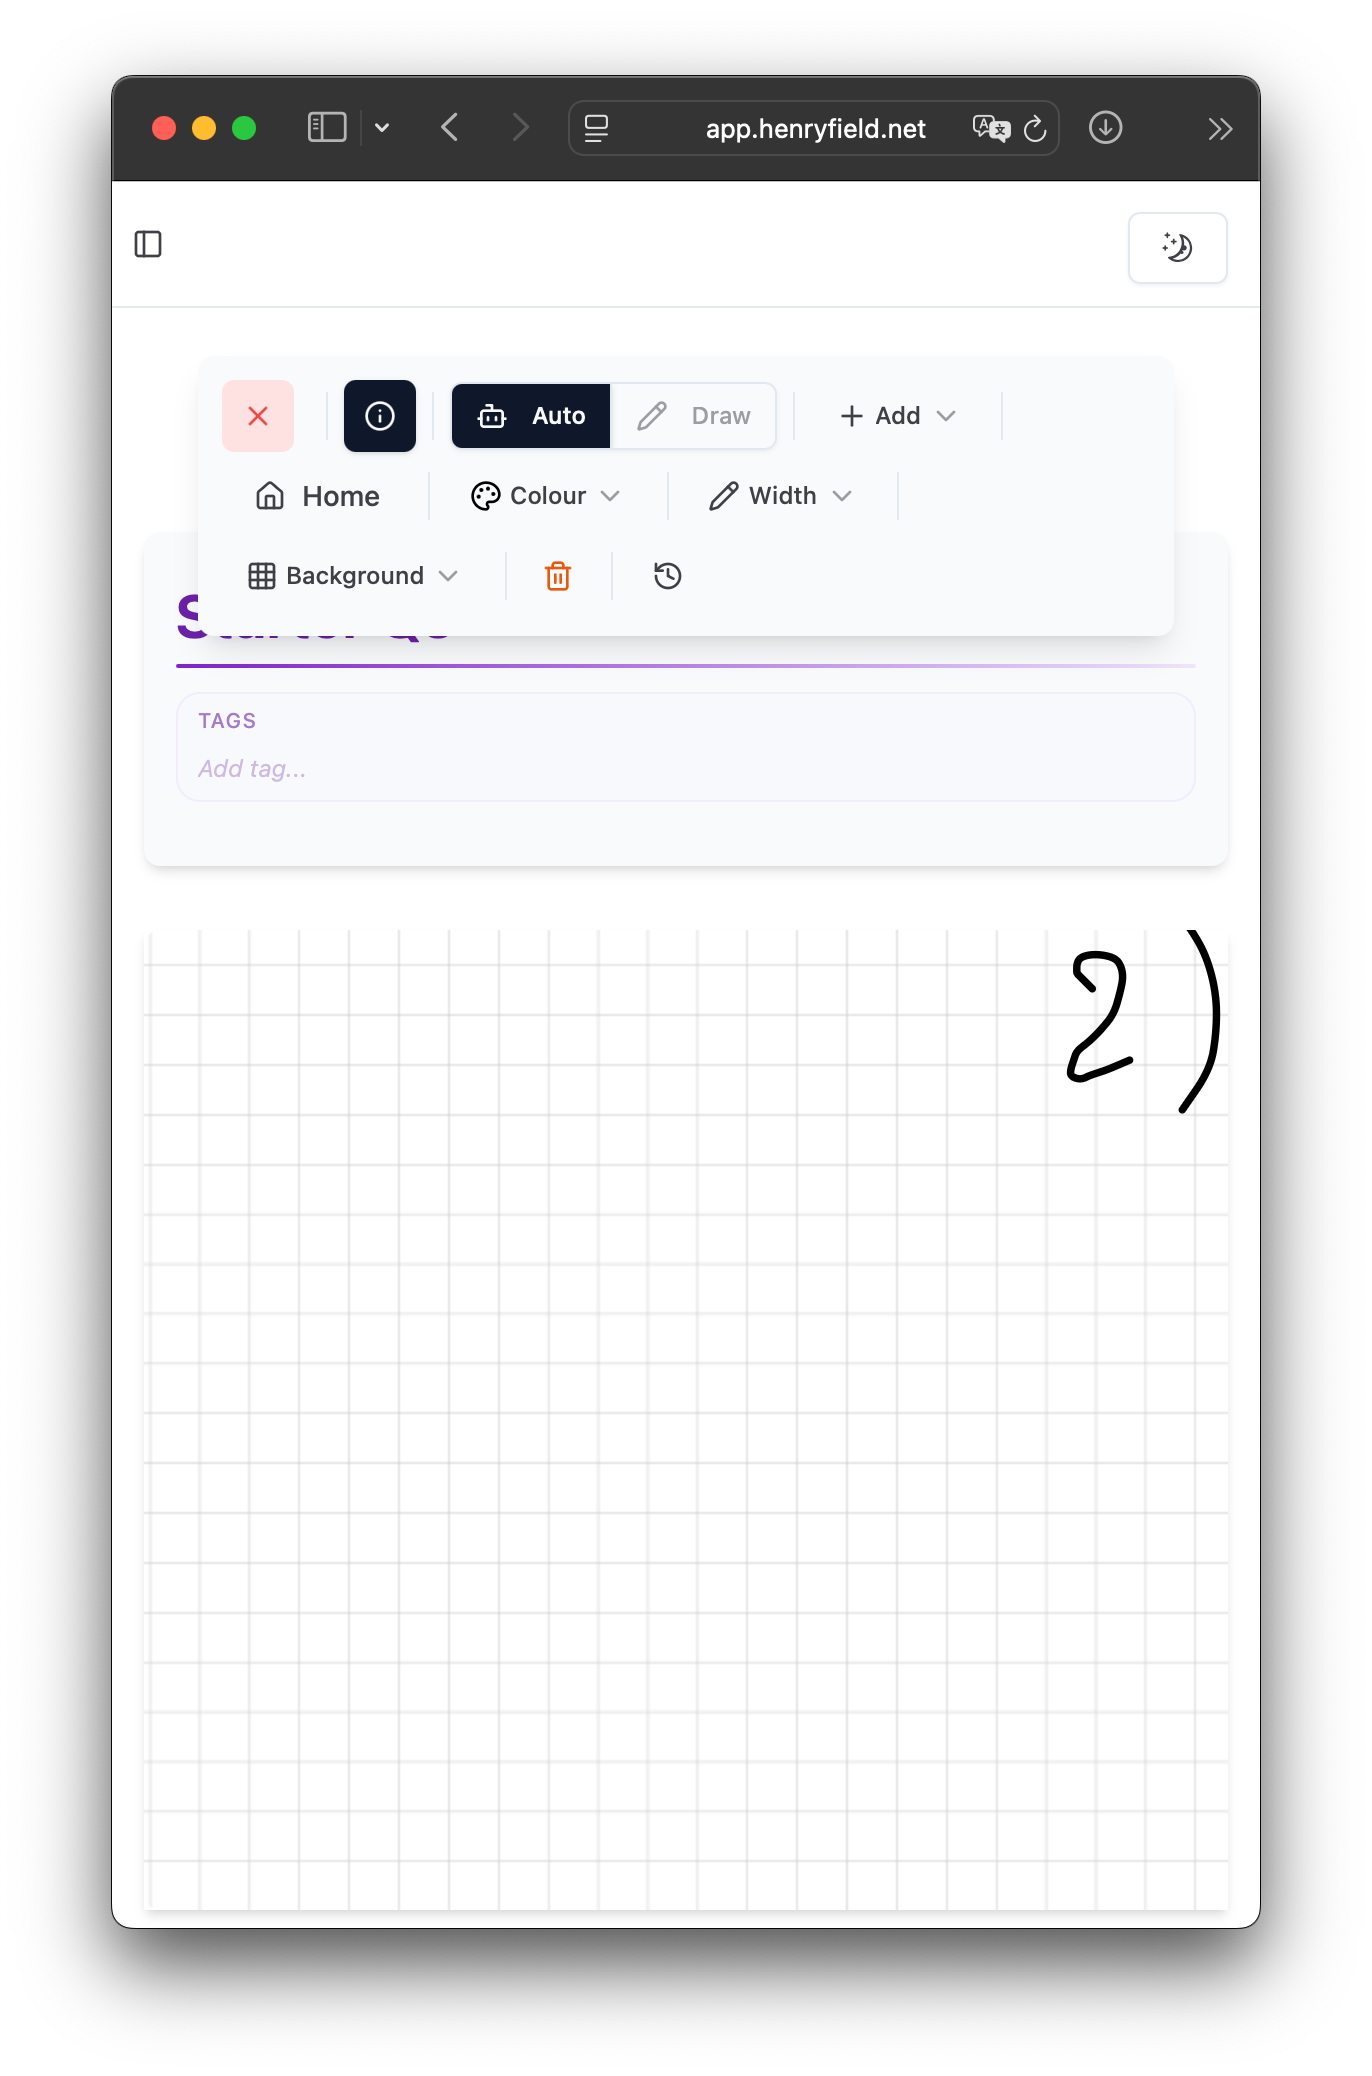
\includegraphics[width=0.8\textwidth]{Diary/33_WC_16-6-25/media/beforeWrap.png}
    \caption{Toolbar wrapping around the screen}
\end{figure}

To rectify this I redesigned it with a number of 'breakpoints' in mind, this system gauges the width of the screen and displays an appropriate number of the most important controls - hiding the rest in a dropdown menu, out of sight but still easy to access. Please see below for examples
\begin{figure}[H]
    \centering
    \begin{minipage}{0.48\textwidth}
        \centering
        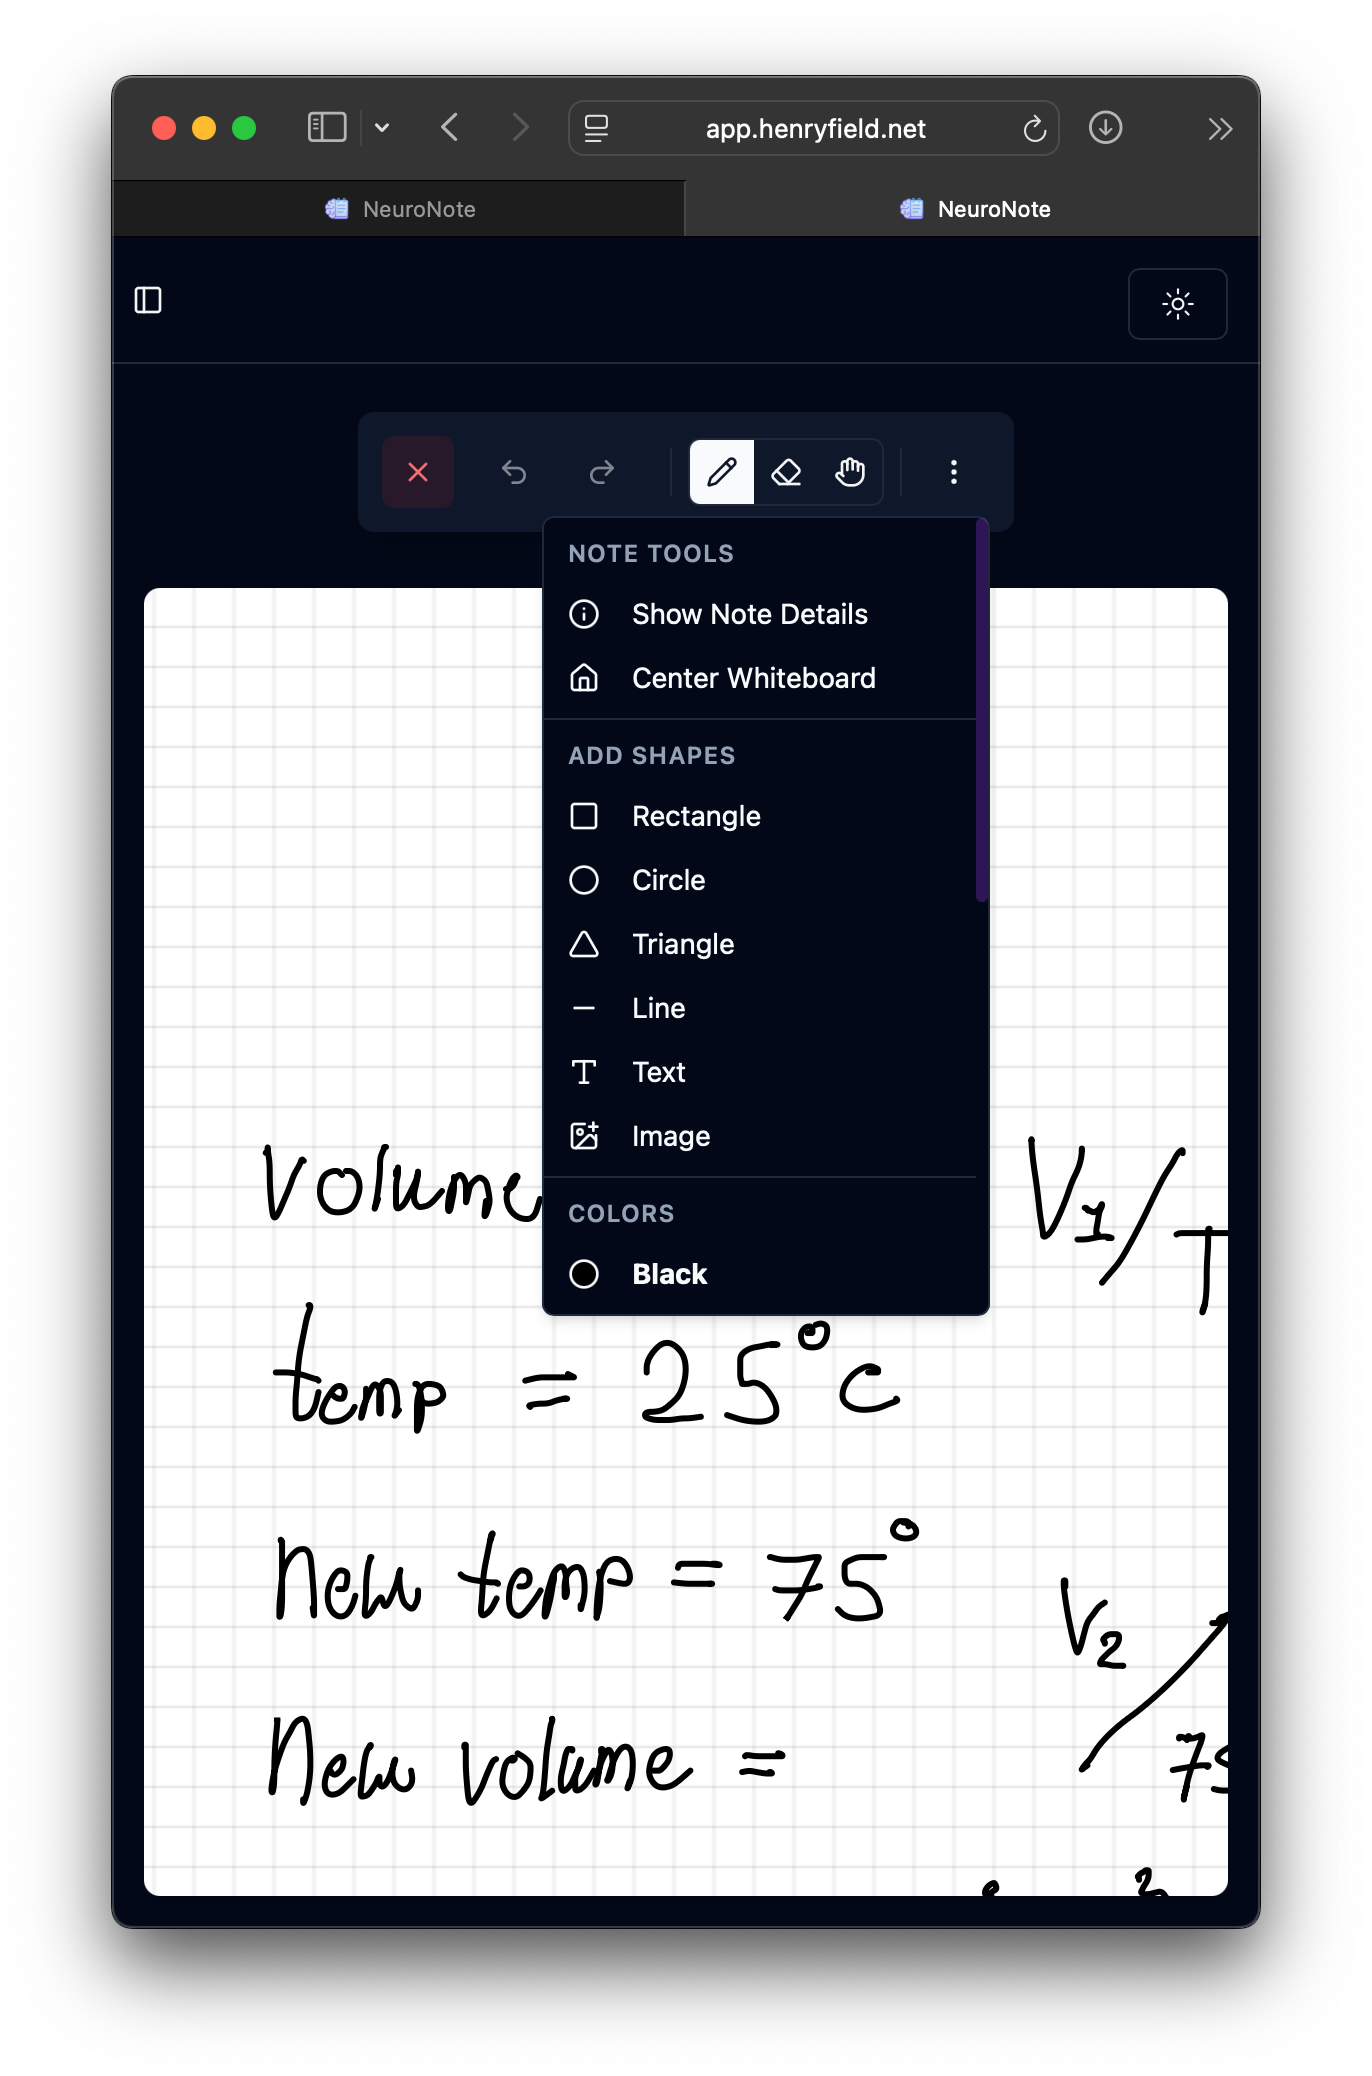
\includegraphics[width=\textwidth]{Diary/33_WC_16-6-25/media/whiteboardafter.png}
        \caption{Whiteboard toolbar after redesign}
    \end{minipage}\hfill
    \begin{minipage}{0.48\textwidth}
        \centering
        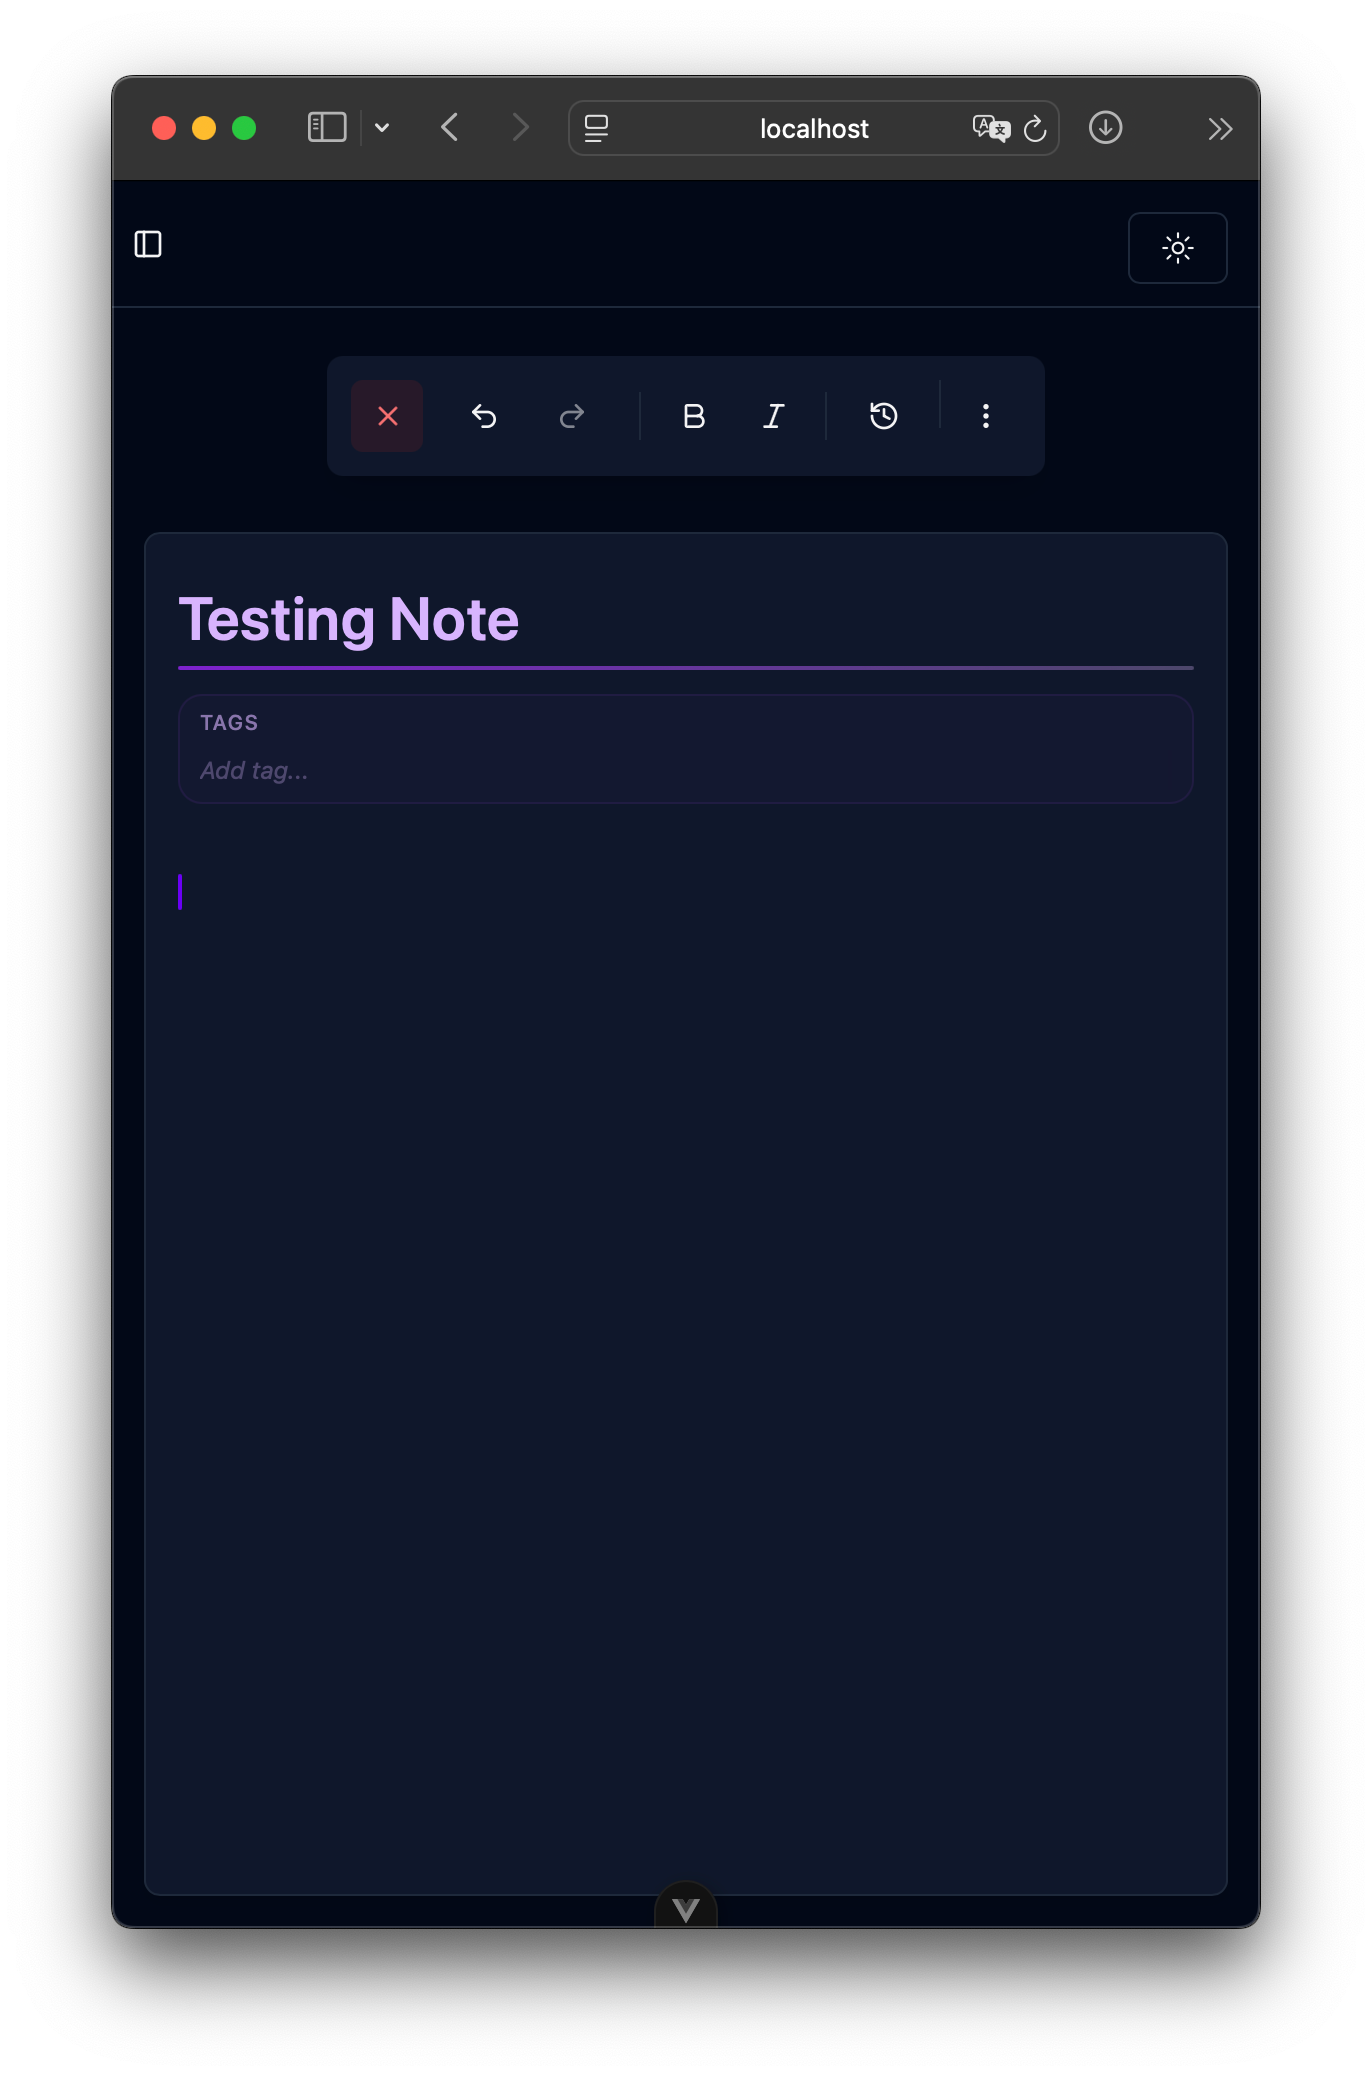
\includegraphics[width=\textwidth]{Diary/33_WC_16-6-25/media/documentAfter.png}
        \caption{Document toolbar after redesign}
    \end{minipage}
\end{figure}

Next I focused on the way my software handles poor internet connectivity, currently any time a connection fails (which can be frequent if travelling) my code displays an error to the user which they must click past to continue. Whilst this is effective in reducing data loss as users cant continue to enter information I have made this slightly more tolerant by allowing for 10 failed attempts to connect before throwing an error, this roughly 2 second tolerance results in a fewer user distractions whilst still minimising potential data loss and is a nice feature for those who are travelling whilst working.

Next I added a few 'fallback designs' for buttons and artwork that will be displayed if the user is unable to access certain resources (I had this appear in testing whilst in school / office environments due to web filtering)

I made a couple of changes in icon sizing so that users with very high bowser scaling multipliers can still fully use the software instead of having their screen covered with the introduction banner / artwork


\subsection*{Plans for next week:}
Next week I will be launching my project to my waiting list and collecting feedback. I will probably face some technical challenges however i am confident that i will be able to solve them efficently thanks to my robust system design and i will ensure i docuement any challenges faced within my diary entry.s